\chapter{Graphic Design}

In this thesis I present the implementation of the student module. In the student module I will implement the following features in priority order:
\begin{enumerate}
	\item see general information about the classes
	\setcounter{enumi}{0}
	\item see the results
	\item list of commits and tagging a commit as final version
	\setcounter{enumi}{1}
	\item set new password, e-mail and SSH public key
	\item summarized view of student's grades
\end{enumerate}

The features with priority level 1 are mandatory, because without these features the portal will be useless for the students.

The features with priority level 2 are important, but the portal is not useless without it. The students can still tag a commit with a Git client, or merge the final commit with the master branch to make it the master branch's last commit. 

The features with priority level 3 are not important, but can be useful for students. The portal is useful without this feature, because the students can check their results on the educational event's page.

In \refstruc{7-test} I will test the features with priority level 1 and 2.


\section{Design Sketches}
To be able to draw design sketches, we need to know when will a user login to use the Educational Support System and what kind of information is he looking for. As a student, there are 5 possible scenarios:

\begin{enumerate}
	\item Before a laboratory
	\begin{itemize}
		\item To get information about the laboratory
		\begin{itemize}
			\item When will it be
			\item Where will it be
			\item Who will be the teacher
		\end{itemize}
		\item To read general information about the course
	\end{itemize}
	
	\item During a laboratory
	\begin{itemize}
		\item To upload an SSH public key
		\item To get his Git remote URL
	\end{itemize}
	
	\item After a laboratory, before the deadline for submitting the homework
	\begin{itemize}
		\item To see the date of the deadline
		\item To see how much time is left until the deadline
		\item To see the pushed branches, commits and tags
		\item To tag a commit as final version
	\end{itemize}
	
	\item After a laboratory, after deadline
	\begin{itemize}
		\item To check his grades
		\item To check his reviews
		\item To check the evaluator's name
	\end{itemize}
	
	\item Other scenarios
	\begin{itemize}
		\item To set a new e-mail address
		\item To set a new password
		\item To change his mailing list subscription
		\item To change his e-mail notification subscription
		\item To see a summarized table of his grades
	\end{itemize}
	
\end{enumerate}

With the scenarios and list of actions, we can see how many pages is needed for the student modules and how many states will one page have. 

\emph{Before laboratory:} For these information I will use only labels \see{fig:before}.

\emph{During laboratory, after laboratory and before deadline:} For the information, like deadline and entry test grade I will use labels. For the list of commits I will use a dropdown menu. When the page is loaded, the last final commit will be the chosen one. If the user did not chose a final commit before, the last commit in the master branch will be the chosen one \see{fig:during}.

\emph{After laboratory and after deadline:} For these information I will use labels. The reviews can be long, and I want to keep the design simple. Because of this, there will be a size limit for the label on the view, and the rest of the text will be hidden with an ellipsis. The user can click on the text to show the rest of the review in a pop up window \see{fig:after}.

\emph{Other scenarios:} The new e-mail address, password and SSH public keys will have input fields. The subscription will be changeable with check boxes \see{fig:settings}. The summarized view will be a simple table with the grades in it \see{fig:results}.

\emph{Menu:} Because the user is looking for a specific set of information, the page will only contain the important information, and the previous, but still relevant information will be accessible with tabs on the laboratory page. To be able to switch between the pages, I will use a navigation bar on the top of the page. The bar will have the logo of the portal and one button for each pages.

I drew sketches \see{appendix-design-sketches} for every state with placeholder data. 

\section{Design template}

To show only a specific set of information I have decided to use a minimalist design. A minimalist design is a clear design, focusing on typography, space, color and basic design elements. This way the portal will show as much information as the user needs with as few elements as possible. 

To look for templates and ideas I read the Designmodo blog~\cite{Designmodo} and checked all the popular websites, e.g., Facebook, Github, Twitter and Medium. Designmodo also have purchasable website builders, like Slides~\cite{Designmodo-slides}, but I prefer the simple design of the Bootstrap elements~\cite{Bootstrap}. 

Bootstrap is a free and open source HTML, CSS and JS framework to create responsive design. It was originally a part of Twitter as Twitter Blueprint, but in 2011 it was released as an open source project. Bootstrap contains elements for responsive web design and mobile design. Bootstrap 4 alpha was launched in August 2015 alongside with a new side project, Official Bootstrap Themes~\cite{Bootstrap-themes}. Bootstrap Themes are purchasable redesigned collections of Bootstrap components with new components and plug-ins. Although I really like these themes, I will use the free components, because it does not worth buying any theme if I will change some parts of the included components. 

\subsection{Colors}

After deciding what kind of design framework will I use, I had to chose the colors of the portal. Both the Budapest University of Technology and Economics~\cite{BME-Arculat}~\cite{BME-Arculat-Intranet} and the Faculty of Electrical Engineering and Informatics~\cite{VIK-Arculat}~\cite{VIK-Arculat-PDF} have their own Visual Identity Guidelines. A visual identity guideline contains the description of which color is the official color of the institution and in what kind of text which fonts and why that font should be used.

I consulted with my advisor, Sándor Gajdos and he told me that I should not follow any of these visual identity guidelines. Following any of the strict guidelines can be a problem in the future, if anyone would like to use this portal for another course that does not belong to the faculty or the university. Based on a subjective opinion I have decided to use green as the main color of the portal. I used the Google Color palette~\cite{google-color-chart} to choose a nice green, changed it a bit, and I got the final color, \#2a623d.

\newpage
\section{Final Graphical Design}

\begin{figure}[!ht]
	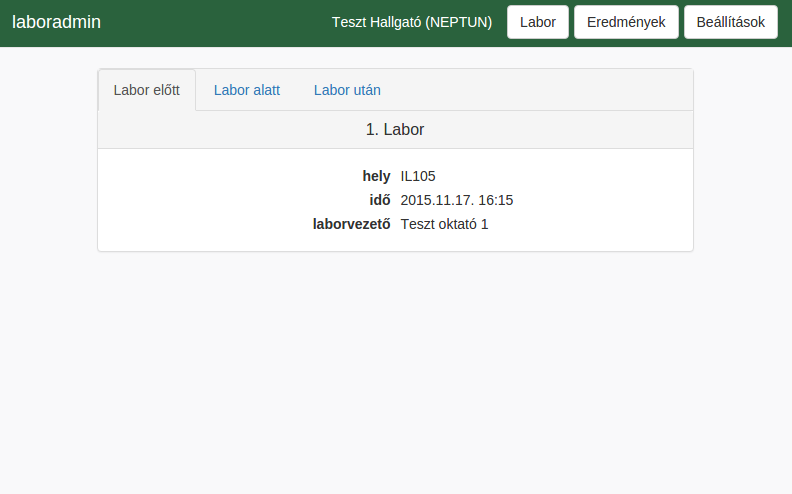
\includegraphics[width=\textwidth]{figures/design/labor_elott.png}
	\caption{Before laboratory}
	\label{fig:before}
\end{figure}

\begin{figure}[!ht]
	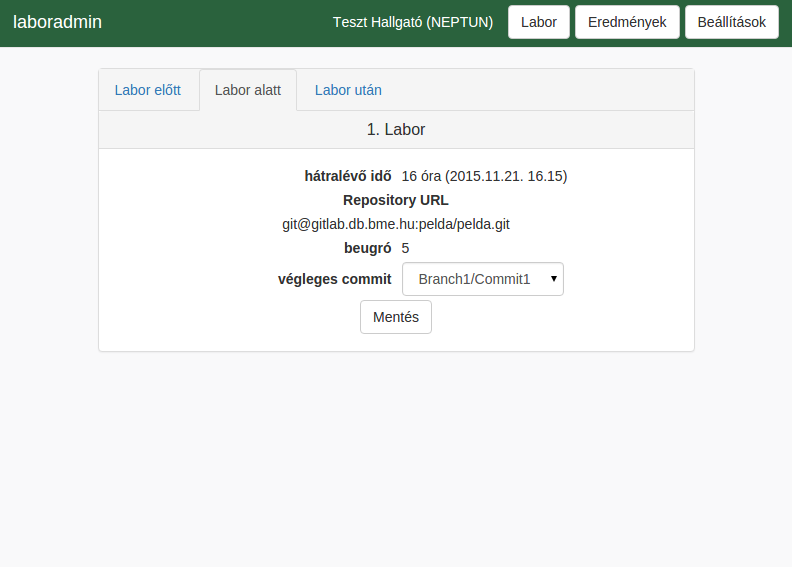
\includegraphics[width=\textwidth]{figures/design/labor_alatt.png}
	\caption{During laboratory}
	\label{fig:during}
\end{figure}

\begin{figure}[!ht]
	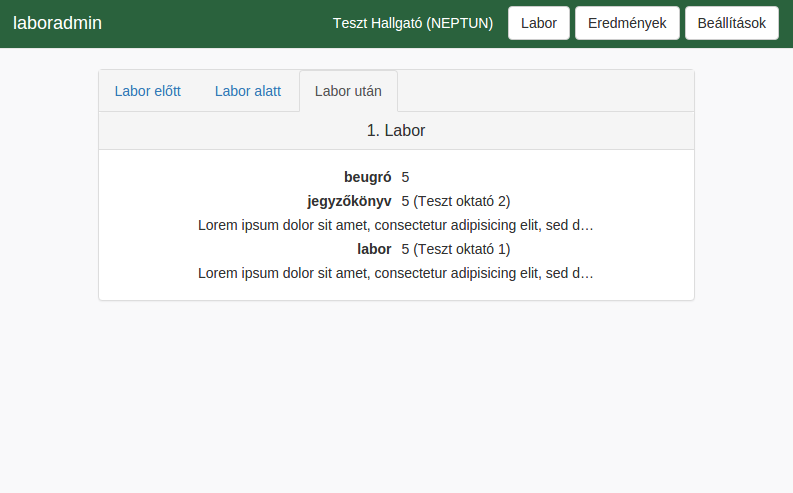
\includegraphics[width=\textwidth]{figures/design/labor_utan.png}
	\caption{After laboratory}
	\label{fig:after}
\end{figure}

\begin{figure}[!ht]
	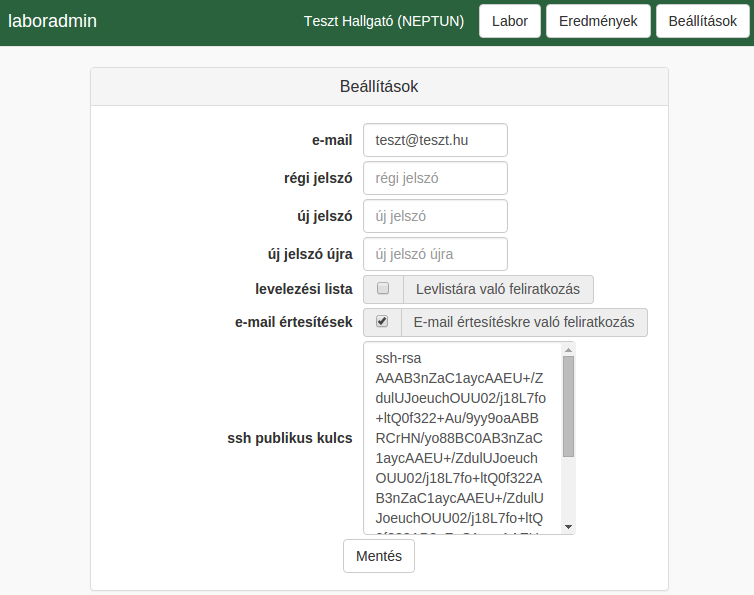
\includegraphics[width=\textwidth]{figures/design/beallitasok.png}
	\caption{Settings}
	\label{fig:settings}
\end{figure}

\begin{figure}[!ht]
	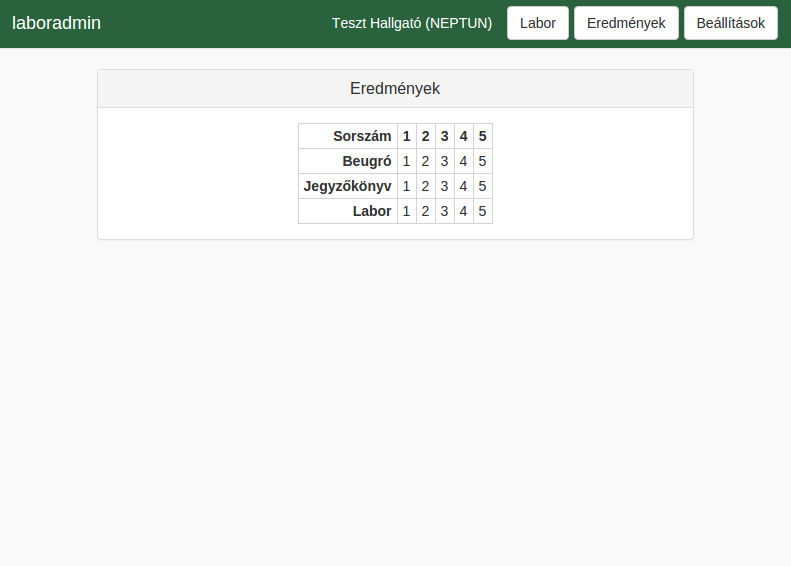
\includegraphics[width=\textwidth]{figures/design/eredmenyek.png}
	\caption{Summarized results}
	\label{fig:results}
\end{figure}

\todo{popup screenshot}

\todo{életlenséggel valamit csinálni kell, hogy fog ez kinézni nyomtatva?}